\section{Проектрирование общей части}
Прежде чем пристпать к непосредсвенной реализации индивидуальной части проекта, была разработана
общая часть проекта. В ней входит диаграмма вариантов использования, концептуальная диаграмма классов и некоторые сценарии.
Диаграмма прецедентов (Use case diagram, диаграмма вариантов использования)~-- диаграмма, на которой отражены отношения, 
существующие между экторами и прецедентами.
Основная задача — представлять собой единое средство, дающее возможность заказчику, конечному пользователю и разработчику совместно
обсуждать функциональность и поведение системы.

Сущности, с которыми взаимодействует система в процессе своей работы, называются экторами, причем каждый эктор ожидает, 
что система будет вести себя строго определенным, предсказуемым образом. В качестве экторов могут выступать человек или 
другая система, подсистема или класс, которые представляют нечто вне сущности.
Прецедент (use-case) - описание отдельного аспекта поведения системы с точки зрения пользователя.
В данном проекте диаграмма прецедентов выглядит так:

\begin{figure}[h]
\centering
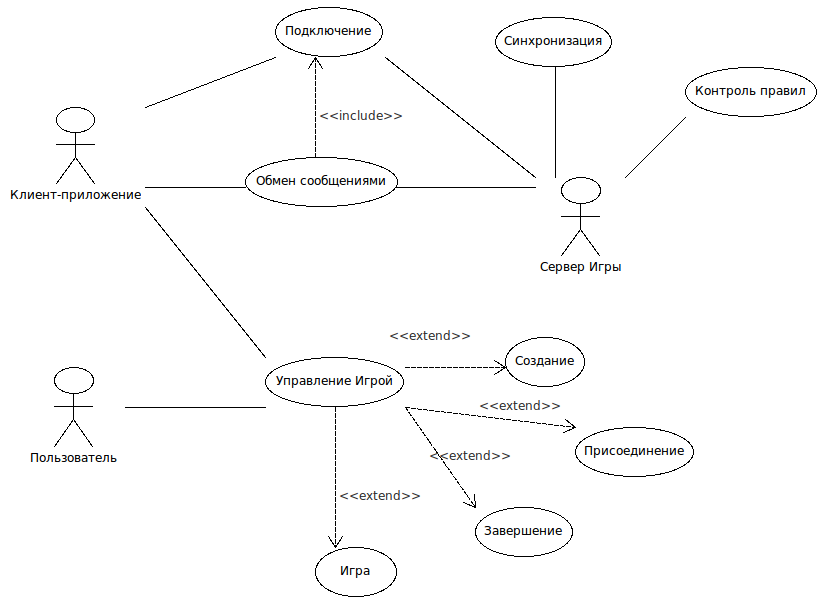
\includegraphics[width=18cm]{images/use.png}
\caption{Диаграмма прецедентов}
\label{fig.0}
\end{figure}

На данной диаграмме видно, что взаимодействие игроков и все их действия осуществляються через сервер игры, который
занимается синхронизацией действий игроков (т.е. чтобы игроки видели перемещения кораблей друг друга)
и проверкой соответсвия их действий правилам игры. Под ролью поьлзователя на данной диаграмме понимается 
чеьловек, который взаимодействует с данным приложением.

\endinput
